%%%%
%%%%
%%%%
\chapter{Summary of applied technologies}
%%%%
%%%%
%%%%

\section{Programming languages and build tools}

We use multiple languages in the framework. 
Xtend is used for the design time utilities in the framework, as its useful for model transformations and template-based code generation.
It is used to process the models and generate the monitoring components. 
The monitoring components are generated as \cpp{} code.
The generated code depends on a library written in \cpp{}, which is also a part of the framework.
The generated code and the library is written in \cpp{} because it can be used in various platforms from embedded systems to high powered computers, or virtual machines in clouds.


\subsubsection{XTend}
The design time tools of the framework are implemented in Xtend\cite{xtend}, which is an extended dialect of Java, with features improving its usability.
Xtend is useful for model transformations, as it provides easy syntax for Java Stream API-like features, which we use extensively as design part tools transform the design artifacts into code in several steps.

Xtend is also useful for implementing template-based code generators. 
Between two \texttt{'''} we can write template expressions.
An example can be seen from the code in \autoref{fig:xtend}, which is a generator for a \cpp{} \texttt{operator==} of a class.


\begin{figure}[H]
	\begin{center}
		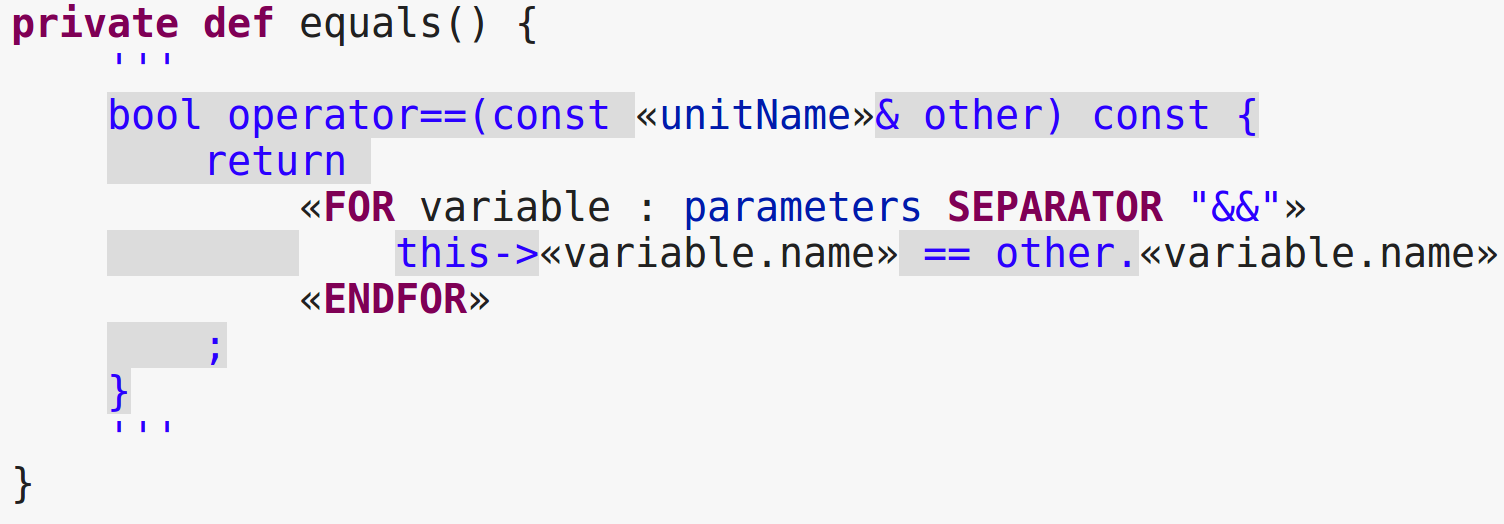
\includegraphics[width=0.8\textwidth]{figures/xtend.png}
		\caption{Template expressions with useful syntax highlight }
		\label{fig:xtend}
	\end{center}
\end{figure}

\texttt{equals} is a function returning a StringBuilder.
Variables between guillemet symbols (\texttt{<<} and >>) are replaced by their value in the string. 
We can also use for loops (<<FOR>> \dots{} <<ENDFOR>>). or conditional expressions (<<IF cond>> \dots{} <<ENDIF>>).
Indentation of the generated code is highlighted, and indentation is handled nicely, so the generated code itself can look good. 
Although this aspect of the generated code is not important for the user of the framework, it was extremely useful in the development process for debugging. 

\subsubsection{\protect\cpptt }

As modern \cpp{} is used in the framework, compiling the code requires a compiler supporting the \cpp{}14 standard.
We use various of modern \cpp{} elements:
\begin{itemize}
	\item Threading -- As the generated monitoring code is integrated into a multi-threaded system, we use \texttt{std::thread}, \texttt{std::mutex}, etc.\ to handle the threads and concurrency
	\item Smart pointers are used for safe resource handling in the framework
	\item Lambda functions also used in the generated code to improve the usability of the framework.
\end{itemize}
The framework library also uses \cpp{} templates to handle generated classes, this feature of C++ is extremely useful to integrate the generated code into the framework at compile time. 

\subsubsection{ Make, CMake }

To build the generated sources and the \cpp{} libraries we developed, we use Make and CMake utilities. 

Make is a low-level build automation tool. 
The build is configured by a file called the Makefile.
A Makefile consists of rules. 
A rule has targets (The artifacts generated by the rule), dependencies (artifacts, that must be created to run the rule), and a list of commands, that creates the target artifacts. 
From this declarative configuration file Make can decide the order which commands to run in which order to create a target artifact or multiple target artifacts.
If only some files changes Make only executes the required commands based on timestamps of the files.

As Makefiles are platform dependent\footnote{The commands generating the artifacts are platform dependent}, we use CMake.
CMake is a higher level tool for build automation. 
It is cross-platform, as CMake configuration files are processed and compiled into project files, such as Visual Studio, or Xcode projects, or build scripts for Make or NMake.

\section{Frameworks}

\subsubsection{Protocol Buffers (Protobuf)}
Protocol Buffers (Protobuf) are a language-neutral, platform-neutral extensible mechanism for serializing structured data \cite{protobuf}. 
We use Protobuf to serialize application messages to a concise binary format.

Protobuf can be used by defining the message structure in \texttt{.proto} files and generating code from them to various languages. This code provides tools for creating, altering, serializing and deserializing messages.

\subsubsection{DDS -- Data Distribution Service}

DDS~\cite{DDS} is a data exchange standard for real-time systems. 
Its usage is publish-subscribe based.
Topics can be defined, where the user of DDS can publish data, or subscribe to get notified about data changes. A topic is a relation (Table with columns and rows with unique keys identifying a row).

We use DDS to synchronize object and reference creation between partial models of the system.


\subsubsection{EMF -- Eclipse Modeling Framework}

Eclipse Modeling Framework is a modeling framework and code generation facility for building tools and other applications based on a structured data model.\cite{emf}.

EMF defines a UML dialect called Ecore, which is presented in \autoref{chapter:emf}. Ecore is used to provide the metamodel of the CPS's live model.


\subsubsection{\protect\viatra{} }


\viatra{} \cite{viatra} is a framework for model transformations and model querying. 
It provides VQL (Viatra Query Language), a language for graph pattern definition. 
Monitoring rules of the CPS are defined in VQL, \autoref{chapter:vql} shows how VQL is built up.
\viatra{} can use local search-based and incremental algorithms~\cite{viatra-incremental} to provide matchings for graph patterns. 

In the framework, we used the local search planner of \viatra{}~\cite{bur-marton-msc}. We extended this planner to create plans for distributed query execution.





